% Template for 61st conference for non-peer-reviewed articled
\documentclass[convention]{aesconf}

% Graphics path
\graphicspath{{./}{figures/}}

% UTF-8 encoding is recommended but use one that works for you.
\usepackage[utf8]{inputenc}

% Highly recommended package for better looking text automatically.
\usepackage{microtype}

% Natbib is used for more control on citations. You can use other moderd
% bibliography packages but please try to match the provided style.
\usepackage[numbers,square]{natbib} 


% These are useful for different purposes.
\usepackage{color}
\usepackage{url}


% The full title of the paper
\title{Audio Source Localization as an Input to Virtual Reality Systems}

% Put the authors in order here. The number in brackets define the corresponding affiliation.
\author[1]{Agneya A. Kerure}
\author[1]{Jason Freeman}

% Affiliations go here
\affil[1]{Georgia Institute of Technology}

% Correspondece should include the corresponding author's name and e-mail address
\correspondence{Agneya A. Kerure}{kerure.agneya@gatech.edu}

% These are used for headers. Anything that fits is okay. Please use proper punctuation.

% If there are many authors, please use the form "First author et al."
\lastnames{Kerure and Freeman}

% Short title should describe your topic but not be too long.
\shorttitle{Audio Source Localization in VR}


% This is required and draws the top title
% AES top title. A little bit volatile but should work for now.
\savebox{\AEStop}{%
	\begin{minipage}{\textwidth}%
		\rule{\textwidth}{1.5pt}\\%
		\\%
		\begin{minipage}[c][\iftoggle{convention}{3.2cm}{3.7cm}][t]{0\textwidth}%
			
\includegraphics[width=20mm]{aeslogo.pdf}%
		\end{minipage}%
		\begin{minipage}{\textwidth}%
			\sffamily%
			\begin{center}%
				\LARGE Audio Engineering Society\\%
				\iftoggle{e_brief}{%
				\hspace{3mm}\fontsize{36}{38pt}\selectfont Convention e-Brief \AESEBriefNumber\\%
				}{%
				\iftoggle{convention}{%
				\fontsize{36}{38pt}\selectfont Convention Paper\\%
				}{%
				\fontsize{36}{38pt}\selectfont Conference Paper\\%
				}}%
				\vspace{0.2cm}%
				\large Presented at the \AESConferenceNumber \iftoggle{convention}{Convention\\}{Conference on\\}%
				\iftoggle{convention}{}{\AESConferenceTopic\\}%
				\AESConferenceDate, \AESConferenceLocation%
			\end{center}%
		\end{minipage}\\%
		\vspace{0.2cm}\\%
		\begin{minipage}{\textwidth}%
			\rmfamily\itshape\small	\AESLegalText%
		\end{minipage}\\%
		\\%
		\rule{\textwidth}{1.5pt}%
	\end{minipage}%
}


\begin{document}


\twocolumn[
\maketitle % MANDATORY! 

\begin{onecolabstract}
This paper details an effort towards incorporating audio source localization as an input to virtual reality systems, focusing primarily on games. The goal of this research is to find a novel method to use live audio as an input for level generation or creation of elements and objects in a virtual reality environment. The paper discusses the current state of audio-based games and virtual reality, and details the design requirements of a system consisting of a circular microphone array which can be used to localize the input audio. The paper also briefly discusses signal processing techniques used for audio information retrieval, and introduces a prototype of an asymmetric virtual reality first-person shooter game as proof-of-concept of the potential of audio source localization for augmenting the immersive nature of virtual reality.
\end{onecolabstract}
]

\section{Introduction}
Audio and music have historically been a passive part of video games. Soundtracks that accompany video games are used to captivate the player's attention and incorporate a sense of realism and emotion into the game, but they have rarely been an active part of the game-play mechanism until recently.
Music driven games started out in the form of rhythm based games where the player's sense of rhythm is challenged. These games typically involve a player in performing certain actions in the form of a dance or pressing buttons in a sequence. With the advent of virtual reality, 
Virtual reality rhythm games mostly work in a similar manner but rely on hand held controllers or motion trackers to interact with the rhythmic elements of the game.
Apart from rhythm, there are a few games which use audio from the user as a core mechanism of game-play. These typically rely on features like volume and pitch to control some aspects of the game.
Speech recognition has also been used as an input modality, typically for user interfaces in games.
The use of audio and its properties as an input to games has been very minimal and with the advancement in gaming technology and signal processing prowess of computers, exploration of these possible real-time interactions is warranted.
An important question to consider would be why use audio at all. There are other ways to locate objects and people in a vicinity around a person which include computer vision, infrared tracking, and even GPS. The advantage audio offers is the ability to process the received signal and get vast amounts of information from it, such as timbral and temporal properties, which can be used in different ways in the game with minimal hardware costs.
Virtual reality offers a paradigm which enables interactions in 360$^\circ$. To fully utilize this paradigm, the system involves a circular microphone array which localizes sounds in 360$^\circ$. This enables truly immersive interactions.

\section{Background}
Rhythm based games started out in Japan as electromechanical arcade games where users would press buttons in rhythm to score more points. As time progresses, the required rhythm gets more complicated and increases in speed. These games would also involve more than one player taking turns and pressing buttons.

Mobile-based games have also used audio as an input to control certain aspects of the game. Chicken Scream \footnote{http://www.perfecttapgames.com} is a mobile game in which the user controls the main character by shouting and screaming. The louder the shout, the faster the character moves. Modulation of volume is used as a mechanism to overcome in-game obstacles.

Audio-only games refer to games which can only be played and perceived through sound and acoustics. They were initially developed for the visually impaired community but have huge potential for mobile and multi-player gaming \cite{rober2005playing}. Although these games are limited in the amount of information which can be conveyed to the player, they also have a few advantages over conventional games, such as increased degree of spatial freedom, no necessity of screens and other costly equipment depending upon the game, lower computational complexity and hence less latency, making these games perfectly suited for mobile gaming.

There are many games in the virtual reality category which use music as an input to generate in-game content. Audioshield\footnote{http://audio-shield.com/} and Rockband VR\footnote{http://www.rockbandvr.com/} are the most important examples of this genre. These typicaly use predetermined times which are determined the  music being played to create cues in the forms of game-objects with which the user interacts.

/////////////////Should I add more research here? \cite{Igarashi:2001:VSU:502348.502372}

\section{System}  
This section describes the algorithms and tools used, and the hardware and software requirements of the system.

The localization of sounds is being done by the ReSpeaker Microphone Array which uses it's XMOS XVSM-2000 DSP chip to perform functions like audio source localization through beamforming, vocal activity detection and dereverberation. These functions are built into the microcontroller and are easily accessible on a Windows machine using the HIDAPI protocol.

For pitch detection, the system uses the time-domain based autocorrelation approach. Here the input signal is divided into short frames and the period of a frame is estimated by computing the autocorrelation functions. In this method, the autocorrelation sequence of each frame of the input audio is determined and the time lag corresponding to the strongest peak is used to determine the fundamental pitch period. This technique is most efficient in the mid- to low-frequency range and thus has been popular in speech recognition applications. The autocorrelation function is represented by: 

\[ [R] (t)  = \int_{i=-{\infty}}^{\infty} S_i^*(\tau) S_i(t+\tau) \delta \tau  \]

Octave errors are common in ACF based pitch detectors. This happens particularly with low quality microphones. Fortunately, these errors do not affect our game-play as we do not need accurate pitch tracking and the classifications required by the game are generally very broad.

Certain aspects of the game depend on grouping of frequency bands together. This is done in Unity3D using inbuilt FFT functions which turns input audio into frequency and amplitude components. The audio samples are then grouped together according to their frequencies into 2 "bands" - one containing bass frequencies between 60-200 Hz and one containing mid to high range frequencies between 300-100 Hz.

\subsection{Tools} 
The system includes a microphone array for the capture of audio to estimate the incident audio angle for the HTC Vive Virtual Reality headset which allows users to move in a restricted 3-D space and interact with it using hand-held controllers which are motion tracked. 

The system uses a ReSpeaker 7-channel Circular Microphone Array\footnote{https://www.seeedstudio.com/} which features an XMOS XVSM-2000 DSP chip, providing excellent performance for word detection. It has a small form factor along with an LED ring to show the direction of arrival it detects. 

The development of the game has been done using Unity3D as the main IDE. The system described in this paper uses JUCE \footnote{https://juce.com} to process the input audio from the microphones. This is because Unity does not natively support stereo audio input for processing. The calculated lag values from JUCE are sent to Unity using Open Sound Control(OSC), which is a communication protocol optimized for modern networking technology. Both JUCE and Unity natively support OSC communication.

The speech recognition used in the system is accomplished using the Microsoft Speech Recognition tool for Unity. 

\section{Game Design}
The main aim of the project is to provide a system which would be able to use the location of an audio source in a virtual reality application. The nature of the application can be very varied - from games to test simulations, and from training environments to social interactions. This research will explore the avenue of game design using the provided source localization data. 
First-person shooter games, which involve the user in a weapon-based combat environment, make the best use cases for the proposed system as it would require increased concentration from the user, who would have to anticipate a target object based on their own sense of hearing, thereby increasing their involvement and immersion in the game.

A number of questions arise from this new method of interaction: 
1. How can the behavior of the game objects instantiated by the localization technique be determined? 
2. How is the in-game audio affected by acoustic source localization? 
3. What new avenues does this method of interaction open in terms of game design? 

The answers to most of these questions are subjective as they depends on the type of game being built. The game objects instantiated by the input audio can follow a predetermined path for different directions of arrival. This could be used for puzzle games, which require the user to solve puzzles or mazes using sound and movement. A second approach could be for the instantiated objects to follow a particular game object or direction. This could be utilized by shooter games, making it a bit easier to shoot using sound. The third and easiest approach would be to only instantiate stationary objects based on the direction of arrival. This approach could be more useful for certain non-game applications such as simulation, analysis, and test environments. 

The in-game audio is highly affected by the acoustic nature of the proposed system. It is well known that game audio is an integral part of the gaming experience. This audio is heard through either loudspeakers or earphones. A system which utilizes loudspeakers is bound to produce sound which will be considered as noise in the audio source localization system, thus greatly reducing the accuracy of localization. It is very important to optimize speaker settings in order to utilize this method of interaction for games. A way to do this could be spatializing the speakers evenly around the microphone to avoid directional bias, using ambient audio instead of sounds with sharp onsets to avoid disturbing localization estimation. The use of appropriate microphones is also very important in order to reduce the effects of noise and echoes in the surrounding acoustic environment. 

The author sees this method opening up avenues for many new types of games and experiences. From FPS to puzzles, from games to simulations and sandboxes, from mobile phone to VR headsets -- anything with audio and video capabilities can utilize this method for a variety of applications.

A prototype two player shooting game was designed to utilize audio localization as an input. This utilized a typical asymmetric VR game mechanism in which one player wears the VR headset and the other utilizes a secondary screen to view and play the game. The objective of the game for the VR player is to survive attacks from the second player for as long as possible. The objective for the second player is to defeat the VR player by attacking using his voice - by speaking certain commands which launch projectiles towards the VR player. The VR player can shoot these incoming projectiles using the hand-held HTC Vive controllers, utilizing a bow-and-arrow, and shield mechanism. The projectiles have properties attached to them which are controlled by the properties of the voice of the second player. The pitch of the voice is mapped to the y-axis location i.e the height at which the projectile flies, the volume determines the size and damage of the projectile, and the location of the player with respect to the microphone array determines the x-axis origin of the projectiles.

\subsection{Mechanics and UI}

\begin{figure}[ht!]
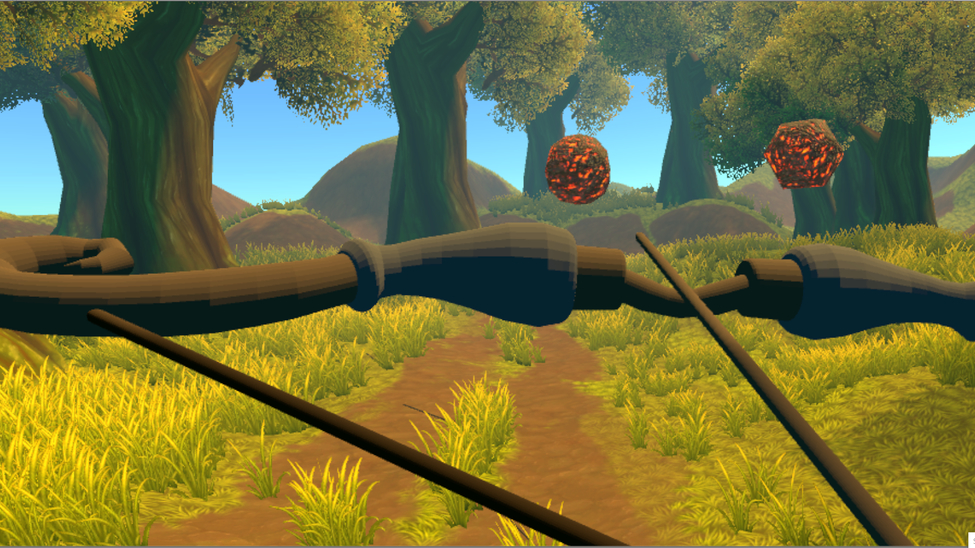
\includegraphics[width=\linewidth]{1}
\caption{In-Game VR Graphics}
\label{auravr} %% The label
\end{figure}


\begin{figure}[ht!]
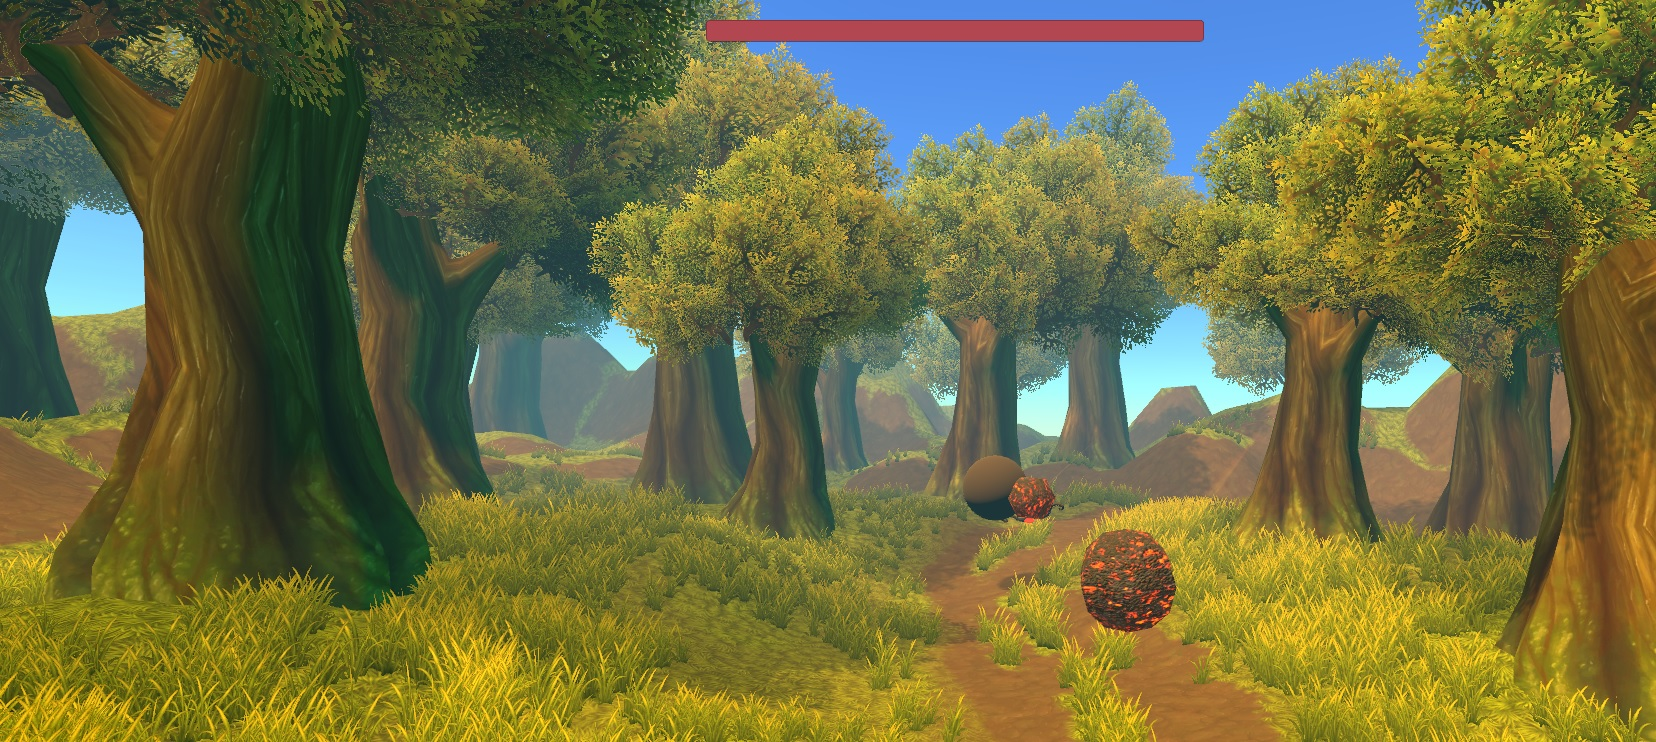
\includegraphics[width=\linewidth]{3}
\caption{Secondary Display (Non VR)}
\label{auravr2} %% The label
\end{figure}

The VR player uses hand-held controllers to shoot at targets using a bow-and-arrow mechanism. The right hand pulls the arrow back keeping the "Trigger" button pressed. To release the arrow, the trigger button is released. The more the arrow is pulled, the farther it will travel. The red indicator on the right hand indicates the current health of the VR player. As soon as the health bar is empty, the game is over.

The non-VR player utilizes voice commands to play the game. The command "Strike" instantiates a target fireball which deals damage to the VR player if hit. The location of the targets depend on the physical location of the non VR-player while shouting the command. The volume of the speaker determines the size and health of the instantiated targets.

After the targets are created, the non-VR player can change their height by speaking in different pitches. The higher the pitch, the more the Y-deviation of the instantiated target in motion. The health of the opponent is visible on the monitor along with his position and the trajectories of the targets.The frequency detected by the microphone is displayed to the right of the opponent health bar. This pitch determines the height at which the targets fly.

As soon as the VR player is defeated, the players would ideally switch roles to compete to see who would last the longest as the VR player and who could best utilize the audio localization and feature extraction mechanism to beat the opponent quickly.

\section{Feedback} 
The game has undergone several iterations of prototyping based on user feedback. Most of the feedback was positive, with people getting excited about the potential of this technology in the world of interactive games and software. There are many robust algorithms which utilize microphone arrays to localize more than one sound source at a time. The test users were excited to learn about the possibilities these sophisticated approaches may provide in the realm of virtual reality experiences.

As for the design of the game, it was noticed that there was  a visible imbalance between the in-game skills required by the VR player and the non-VR player who uses his voice. There was very little skill required by the non-VR player to win the game as he could just keep saying the keyword to generate a large number of projectiles towards the VR player. This helped realize the need to limit the number of projectiles created. There was also a need to restrict potential projectile spawn points so that it is easier for the players to understand the game and how movement was actually correlated to the spawning of the projectiles. 
To increase the skill required and the involvement of audio localization, the non-VR player was given the ability to control the path of the projectile towards the VR player by singing and changing the pitch of his voice - the pitch was directly correlated to the y-axis displacement from the original trajectory. This also provided for a fun experience for the VR user as he now had to try and guess where the opponent would take his projectile and shoot at it. 

An important point of discussion was the use of a real-time key word detection library over a trained classifier, which provided much less latency but also compromised on accuracy. Because of the limited keywords used, it was deemed that a classifier would serve the needs for this game better but due to limitations in time, it was not implemented. The Microsoft keyword detection software, however, does the job fairly decently with acceptable latency.

Another important point of discussion was the decision to use keyword detection over singing voice analysis for the generation of game objects. This is a variation in the type of game-play made possible by the technology. The game in its current form tries to incorporate both keyword detection and singing voice analysis by utilizing pitch detection to move the instantiated projectiles. More complicated and robust singing voice analysis will be utilized in upcoming iterations of the game.

There was an understandable bias towards wanting to be the VR player rather than the one trying to attack using the microphones due to the truly immersible nature of virtual reality. Future enhancements to the audio localization system will attempt to bridge this preference gap by increasing the functionality and intuitive ease of use for the non-VR player.

\section{Challenges}
There were a few main challenges which were addressed in the different stages of development of the system: 
\begin{itemize}
\item Unity not supporting multi channel audio from audio interfaces natively made the use of an external audio manager a necessity. The JUCE C++ library was chosen for this task because of its robust audio handling capabilities.
\item Real-time audio source localization, information extraction, and keyword detection have varying amounts of latency associated with them. Meaningfully mapping this information to instantiated game objects so that it is understood by the players is a challenge.
\item The restrictions introduced on the in-game audio by the acoustic nature of the system present a huge trade-off.
\end{itemize}

\section{Conclusion}
This paper proposes a system which involves audio source localization and signal processing to provide inputs to a virtual reality environment. The use of this system in a prototype game as a proof-of-concept has been discussed, and the hardware and software requirements of the system were mentioned. Design issues and challenges that are associated with this new interaction have also been discussed. 


//~~~~~~~~~~~~~~~~THIS??

The author sees this project as a proof-of-concept for VR and AR headsets with in-built audio source localization capabilities.

\bibliographystyle{jaes}

% Reference to bibliography file.
\bibliography{refs}


\end{document}